\documentclass[slides]{pgnotes}

\title{Basic remoting}

\begin{document}

\maketitle

\tableofcontents

\section{Lab scenario}

\begin{center}
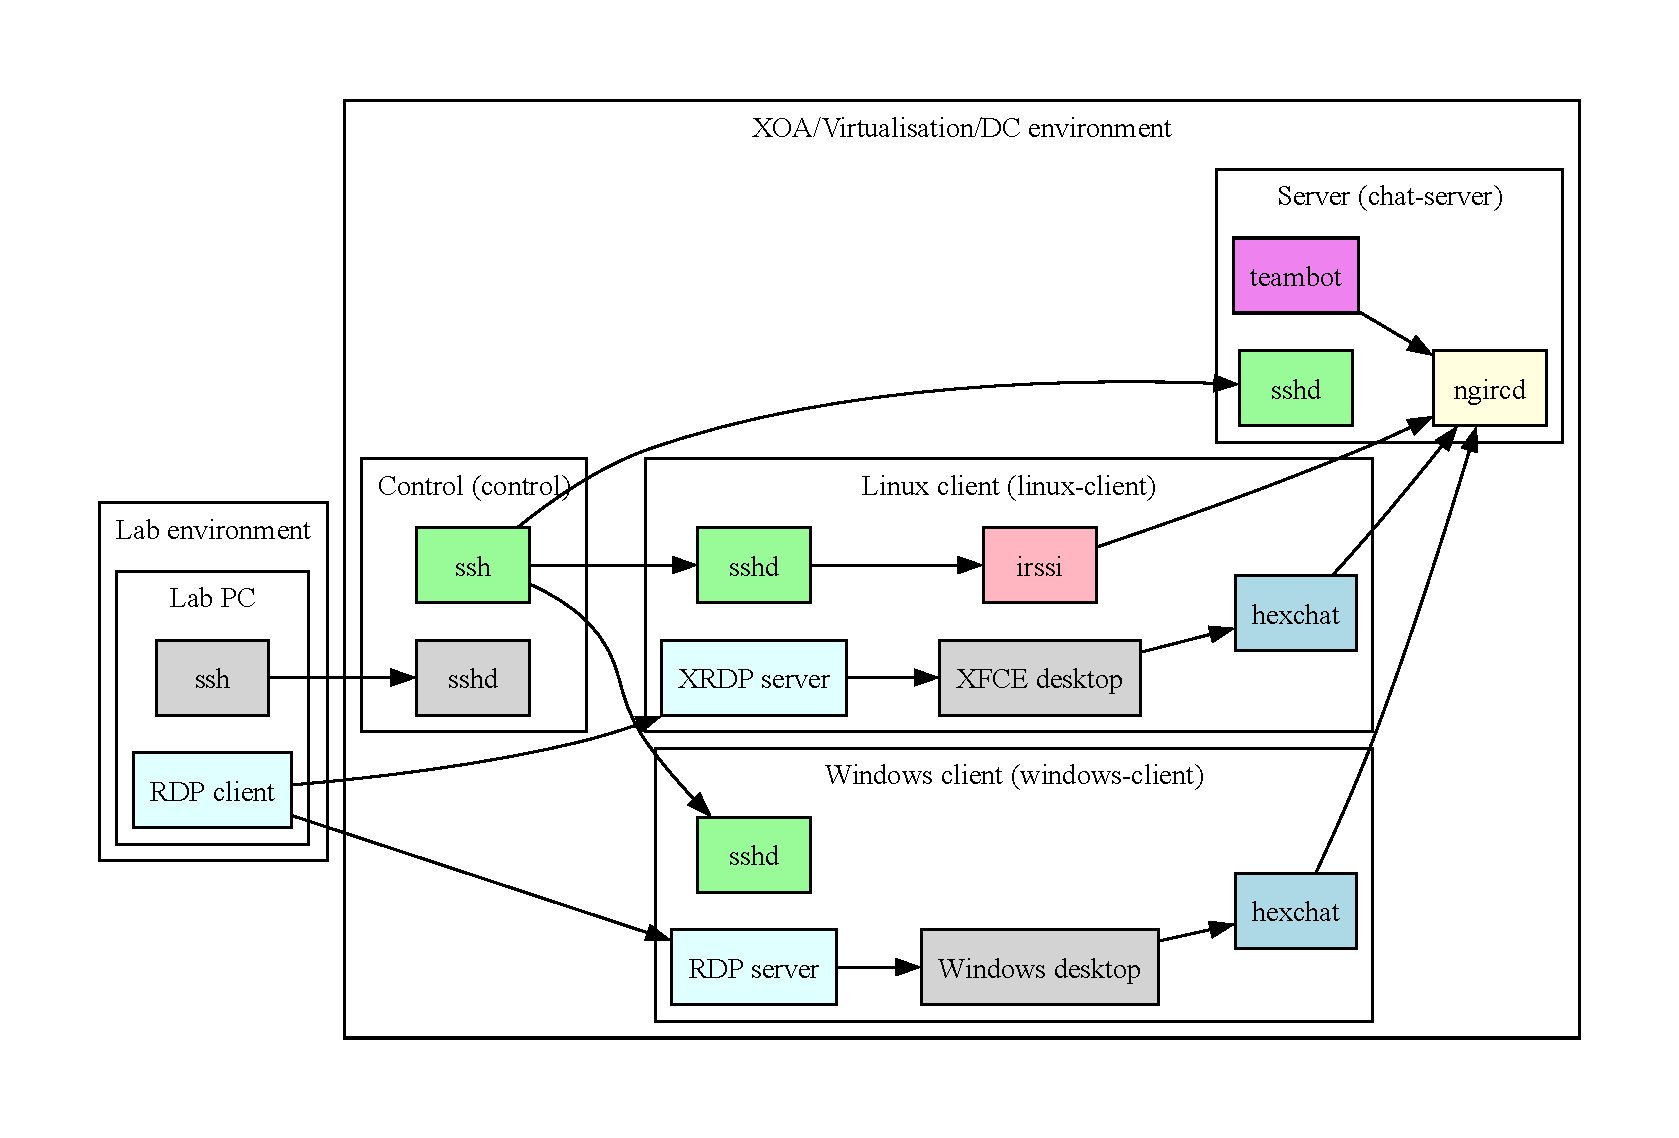
\includegraphics[width=0.7\linewidth]{scenario}
\end{center}

\begin{redbox}{Night class only}
  We will set up the Windows and Linux VMs now on XOA!
\end{redbox}

\section{Remoting}

\textbf{Remoting} refers to a general pattern where we execute commands:
\begin{bluebox}{Participants}
\begin{itemize}
\item from a \textbf{local} (or source) system
\item on a \textbf{remote} (or target) system
\end{itemize}  
\end{bluebox}
Unlike SSH or Telnet remote login, remote command execution is usually driven by the source end.

The source and target systems may differ significantly from each other:

\begin{bluebox}{Heterogenous participants}
\begin{description}
\item[Provisioning] on bare-metal/VM in local/DC, cloud instances, mix.
\item[Operating system] on each
\end{description}
\end{bluebox}


\section{SSH capabilities}

\textbf{SSH} (TCP Port 22) is often used as the means to provide remoting.

\begin{greenbox}{SSH usage patterns}
  \begin{itemize}
  \item Running a full remote shell session (most common usage)
  \item Running a single command
  \item Transferring files (using SFTP)
  \item Port forwarding
  \end{itemize}
\end{greenbox}

The environment exposed over SSH is completely dependent on the \textbf{target} system.


\subsection{SSHD}

SSH is provided by the \textbf{SSH daemon} \texttt{(sshd)} on the remote server.

\includegraphics[width=1.0\linewidth]{sshd}


\subsection{Default Shell}

Normally a connection over SSH invokes a command shell depending on:
\begin{itemize}
\item Default settings in the SSH daemon
  \begin{itemize}
  \item In \texttt{sshd\_config} file
  \item Powershell or CMD in Windows via Registry
  \end{itemize}
\item Connecting user's default shell setting
  \begin{itemize}
  \item Defined in \texttt{/etc/passwd}
  \end{itemize}
\end{itemize}


\subsection{Authentication}

Every SSH connection is associated with a particular user account on the remote system.

The username is passed in the SSH command string:

\begin{description}
\item[In hostname] after the @ sign:
  \begin{itemize}
  \item \texttt{ssh joe@10.2.3.2}
  \end{itemize}
\item[Using the -U parameter] in the command options:
  \begin{itemize}
  \item \texttt{ssh -U joe 10.2.3.2}
  \end{itemize}
\end{description}


\section{Key-based authentication}

\begin{center}
  \includegraphics[width=0.5\linewidth]{key_pair}
\end{center}
  
\end{document}

